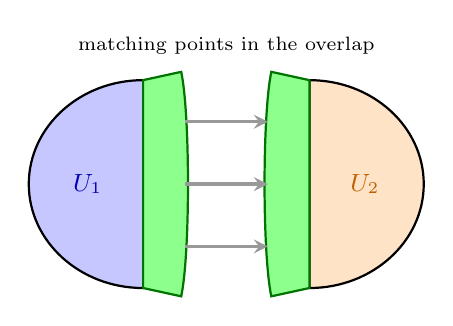
\begin{tikzpicture}[>=stealth, scale=0.88]
  % Two overlapping open patches, each with a collar along its full flat edge
  \draw[thick, fill=blue!22] (-1.2,1.5) arc (90:270:1.65 and 1.5) -- cycle;
  \path[fill=green!45, draw=green!45!black, thick]
    (-1.2,1.5) -- (-1.2,-1.5) -- (-0.65,-1.62)
    .. controls (-0.52,-1.0) and (-0.52,1.0) .. (-0.65,1.62) -- cycle;

  \draw[thick, fill=orange!22] (1.2,1.5) arc (90:-90:1.65 and 1.5) -- cycle;
  \path[fill=green!45, draw=green!45!black, thick]
    (1.2,1.5) -- (1.2,-1.5) -- (0.65,-1.62)
    .. controls (0.52,-1.0) and (0.52,1.0) .. (0.65,1.62) -- cycle;

  \node[font=\small, text=blue!70!black] at (-2.0,0) {$U_1$};
  \node[font=\small, text=orange!75!black] at (2.0,0) {$U_2$};
  \node[font=\scriptsize] at (0,2.0) {matching points in the overlap};

  % Arrows pair points all along the two full-edge overlap collars
  \draw[->, very thick, gray!80] (-0.6,0.9) -- (0.6,0.9);
  \draw[->, very thick, gray!80] (-0.6,0) -- (0.6,0);
  \draw[->, very thick, gray!80] (-0.6,-0.9) -- (0.6,-0.9);
\end{tikzpicture}
